\documentclass[12pt,a4paper]{article} 
\usepackage[utf8]{inputenc}
\usepackage{amsmath} 
\usepackage{amsfonts} 
\usepackage{amssymb} 
\usepackage[all]{nowidow} 
\usepackage[style=authoryear, backend=biber, maxnames=3]{biblatex} 
\usepackage[all]{nowidow} 
\usepackage{hyperref} 
\usepackage[pdftex]{graphicx}
\usepackage[onehalfspacing]{setspace} 

\usepackage{tikz}
\usepackage{standalone}
\usepackage{eurosym}
\usepackage{ntheorem}
\theoremseparator{:}
\newtheorem{hyp}{Hypothese}
\usepackage{dcolumn}
\usepackage{graphics}
\usepackage{graphicx}

\usepackage[english]{babel} % for the language

\usepackage{fullpage} % this and the next one is for 1-inch margin 
%\usepackage{setspace}
%\doublespacing


\addbibresource{bib_file.bib} 
\setlength\parindent{0pt} 

\newcommand{\Title}{Religious people do not discount the future less} 


\newcommand{\Programme}{Corporate Management \& Economics}
\newcommand{\AsssignmentName}{Assignment}
\newcommand{\Name}{Samuel Pertl}
\newcommand{\MatrikelNummer}{000055998}
\newcommand{\Date}{20-12-2016}
\newcommand{\Semester}{Fall Term 2017}
\newcommand{\Supervisor}{Thor Veen}
\newcommand{\Class}{Data Science A}

\begin{document}
\pagenumbering{gobble}
\begin{centering}
\Large \textbf{Quest University} \\
\vfill
\LARGE \textbf{\Title} \\
\vfill
\LARGE \AsssignmentName \\ %Bachelorarbeit
\Large in \\
\LARGE  \Class \\
\vfill
\begin{small}
\begin{doublespace}
	\begin{tabbing}
	Immatrikulationsnummerrrrr\=\kill
	Name:\>\Name\\
	Matriculation Nummer:\>\MatrikelNummer\\
	Semester:\>\Semester\\
	Supervisor:\>\Supervisor\\
	Date:\>\Date
	\end{tabbing}
\end{doublespace}
\end{small}



\end{centering}\vspace{1cm}
\newpage

\pagenumbering{roman}
\tableofcontents
\listoffigures
\listoftables

\newpage

\begin{abstract}
Hello my name is Samuel. I am form Germany and I attend
\end{abstract}
 

\section{Introduction \& Methods}
Introduction (3/4 page), Methods (1 page), 
Results (2 pages) and Discussion (3/4 pages) sections


introduction: intertemporal choice experiment
delay gratification has several beneficial outcomes 
 
Delay gratification could be encouraged by religion as many religions emphasize future rewards instead of immediate gratification such as reincarnation, resurrection and immorality \parencite{carter2012religious}. Furthermore patience has an important role in many religions \parencite{carter2012religious}. Socialization in a religious environment might therefore lead to a more patient behavior resulting in a preferce for a higher later reward instead of a instant gratification \parencite{carter2012religious}.\\
In line with the economic literature the trad-off between instant and delay gratification can be model through an intertemporal choice experiment. In an intertemporal choice experiment participants have to decide between an amount $x$ now and a higher amount $x+y$ later, where $y$ is a positive number.\\ 

% not clear what I mean by future discounting 
To my knowledge three papers have investigated the relationship between religion and future discounting so far. 
 
\textcite{carter2012religious} found that religious people discount have a stronger preference for later reward as their non-religious counterparts and therefore discount future rewards less. Controversial, neither \textcite{thornton2015divine} nor \textcite{benjamin2010religious} observed a significant relationship between religion and discounting of future rewards.\\ 

Based on the controversial findings as well as the scarcity of the previous research more research is needed to to clarify the relationship between religion and discounting of future rewards.\\
Besides this all three studies have major drawbacks. \textcite{carter2012religious, benjamin2010religious} use undergraduate students from the United States as their participants. According to \textcite{henrich2010weirdest} undergraduate students from "Western, Educated, Industrialized, Rich and Democratic" (WEIRD) societies - especially form the USA - are the least representative samples which substantially limits the generalization of their findings. \textcite{thornton2015divine} take this drawback into consideration and recruited their participants on the online labour market M-Turk. Even though, participants from M-Turk are a more representative sample than undergraduates they are not a representative sample since people who work online are just a small fraction of the hole population \parencite{horton2011online}.\
Additionally, all three studies either do not control or just control for very few variables which could have an influence on future discounting.\\

Based on these drawbacks this study uses a representative sample of the German population to investigate the relationship between future discounting and religion and controls for several variables that are associated with future discounting.
Based on the existing literature the research question for the following paper is: 
\begin{hyp}
Religious people discount the future less than non-religious people and have therefore a stronger preference for later rewards as non-religious participants
\end{hyp}

\subsection{Sample} 
The sample consist of a cross section of the German population.\footnote{For a detailed description of the data collection see \textcite{dohmen2010risk}} To measure future discounting each participant took part in an intertemporal choice experiment. For this purpose each participant with 



100 euros "today" and a higher amount $Y$ in 12 months. 

which variables do I use and why do I use them 

\subsection{Methods}
Methods
visualization  
descriptive statistics 
linear regression 
glm: I do not know if I have count data or not 
Question for Monday 

\section{Results}


describe the demographics 
mean age 46 (range 14 - 90) 

religious affiliation: 

Catholic: 31.4 percent
Protestant: 34.8 
A member of a different Christian denomination or religious community: 2.6
A member of an Islamic religious community: 2.2 
A member of another religious community: 0.2 
not a member of a religious community: 28.8 

gender 
female: 53.8
male 46.2 

west/east 
west 77.8 
east 22.2
\subsection{Methods}



I use a significance level of alpha is 5 percent which allows to observe significant results that are not significant under the conventional 5 percent significance level. I do not mention the significance level if not stated otherwise. 

the same applies for ceteris paribus 

\subsection{Visualizing the data }
Visualizing the data with a histogram and a QQplot shows that switching row might not be normally distributed. 
a lot of observations on the very right   
A Shapiro-Wilk normality test supports this impression of a non normal distribution (p-value $< 0.0001$).\\
% try the same but exclude the 21 observations 
\begin{figure}
\scalebox{0.8}{
% Created by tikzDevice version 0.10.1 on 2016-12-17 11:18:50
% !TEX encoding = UTF-8 Unicode
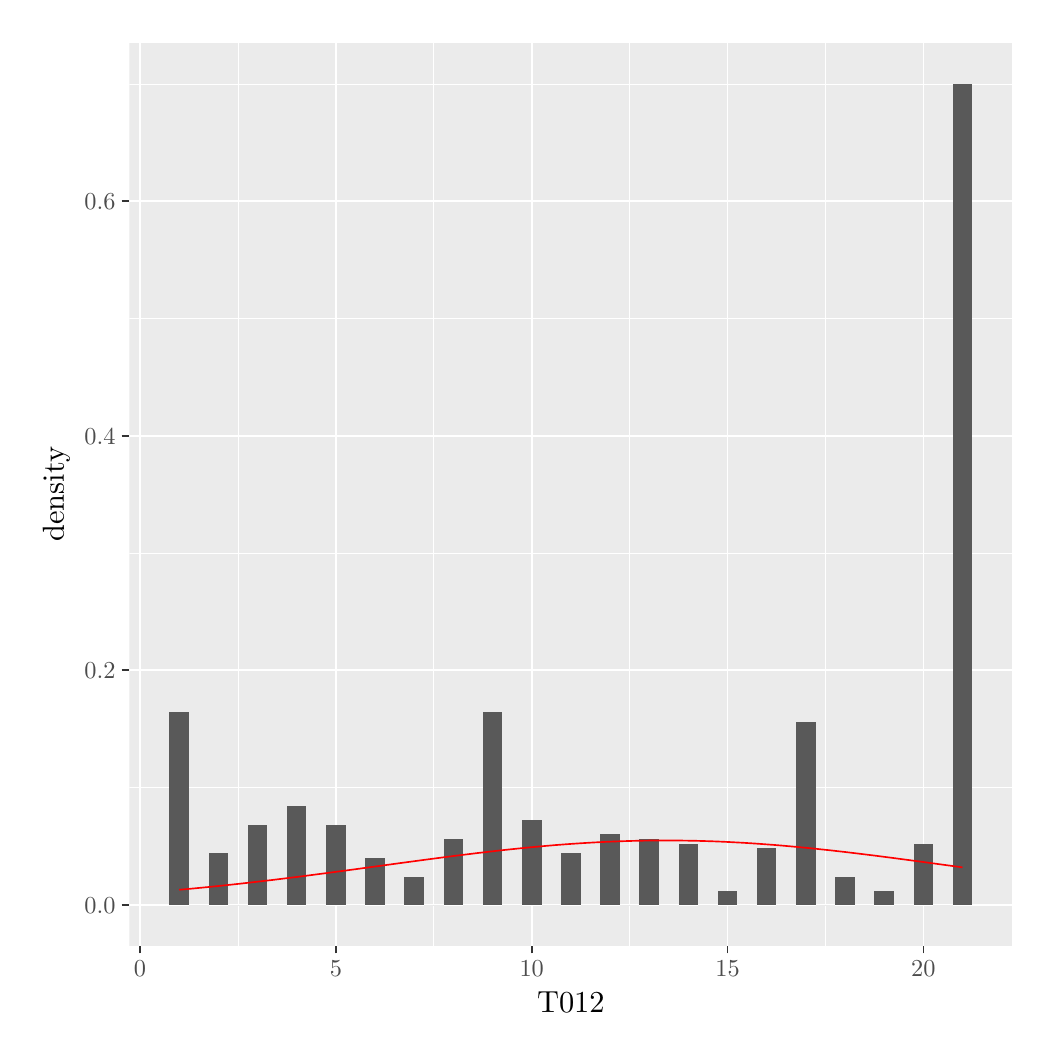
\begin{tikzpicture}[x=1pt,y=1pt]
\definecolor{fillColor}{RGB}{255,255,255}
\path[use as bounding box,fill=fillColor,fill opacity=0.00] (0,0) rectangle (361.35,361.35);
\begin{scope}
\path[clip] (  0.00,  0.00) rectangle (361.35,361.35);
\definecolor{drawColor}{RGB}{255,255,255}
\definecolor{fillColor}{RGB}{255,255,255}

\path[draw=drawColor,line width= 0.6pt,line join=round,line cap=round,fill=fillColor] (  0.00, -0.00) rectangle (361.35,361.35);
\end{scope}
\begin{scope}
\path[clip] ( 36.71, 29.59) rectangle (355.85,355.85);
\definecolor{fillColor}{gray}{0.92}

\path[fill=fillColor] ( 36.71, 29.59) rectangle (355.85,355.85);
\definecolor{drawColor}{RGB}{255,255,255}

\path[draw=drawColor,line width= 0.3pt,line join=round] ( 36.71, 86.79) --
	(355.85, 86.79);

\path[draw=drawColor,line width= 0.3pt,line join=round] ( 36.71,171.53) --
	(355.85,171.53);

\path[draw=drawColor,line width= 0.3pt,line join=round] ( 36.71,256.28) --
	(355.85,256.28);

\path[draw=drawColor,line width= 0.3pt,line join=round] ( 36.71,341.02) --
	(355.85,341.02);

\path[draw=drawColor,line width= 0.3pt,line join=round] ( 75.98, 29.59) --
	( 75.98,355.85);

\path[draw=drawColor,line width= 0.3pt,line join=round] (146.75, 29.59) --
	(146.75,355.85);

\path[draw=drawColor,line width= 0.3pt,line join=round] (217.51, 29.59) --
	(217.51,355.85);

\path[draw=drawColor,line width= 0.3pt,line join=round] (288.27, 29.59) --
	(288.27,355.85);

\path[draw=drawColor,line width= 0.6pt,line join=round] ( 36.71, 44.42) --
	(355.85, 44.42);

\path[draw=drawColor,line width= 0.6pt,line join=round] ( 36.71,129.16) --
	(355.85,129.16);

\path[draw=drawColor,line width= 0.6pt,line join=round] ( 36.71,213.90) --
	(355.85,213.90);

\path[draw=drawColor,line width= 0.6pt,line join=round] ( 36.71,298.65) --
	(355.85,298.65);

\path[draw=drawColor,line width= 0.6pt,line join=round] ( 40.60, 29.59) --
	( 40.60,355.85);

\path[draw=drawColor,line width= 0.6pt,line join=round] (111.37, 29.59) --
	(111.37,355.85);

\path[draw=drawColor,line width= 0.6pt,line join=round] (182.13, 29.59) --
	(182.13,355.85);

\path[draw=drawColor,line width= 0.6pt,line join=round] (252.89, 29.59) --
	(252.89,355.85);

\path[draw=drawColor,line width= 0.6pt,line join=round] (323.65, 29.59) --
	(323.65,355.85);
\definecolor{fillColor}{gray}{0.35}

\path[fill=fillColor] ( 51.22, 44.42) rectangle ( 58.29,113.91);

\path[fill=fillColor] ( 58.29, 44.42) rectangle ( 65.37, 44.42);

\path[fill=fillColor] ( 65.37, 44.42) rectangle ( 72.45, 63.06);

\path[fill=fillColor] ( 72.45, 44.42) rectangle ( 79.52, 44.42);

\path[fill=fillColor] ( 79.52, 44.42) rectangle ( 86.60, 73.23);

\path[fill=fillColor] ( 86.60, 44.42) rectangle ( 93.68, 44.42);

\path[fill=fillColor] ( 93.68, 44.42) rectangle (100.75, 80.01);

\path[fill=fillColor] (100.75, 44.42) rectangle (107.83, 44.42);

\path[fill=fillColor] (107.83, 44.42) rectangle (114.90, 73.23);

\path[fill=fillColor] (114.90, 44.42) rectangle (121.98, 44.42);

\path[fill=fillColor] (121.98, 44.42) rectangle (129.06, 61.37);

\path[fill=fillColor] (129.06, 44.42) rectangle (136.13, 44.42);

\path[fill=fillColor] (136.13, 44.42) rectangle (143.21, 54.59);

\path[fill=fillColor] (143.21, 44.42) rectangle (150.29, 44.42);

\path[fill=fillColor] (150.29, 44.42) rectangle (157.36, 68.15);

\path[fill=fillColor] (157.36, 44.42) rectangle (164.44, 44.42);

\path[fill=fillColor] (164.44, 44.42) rectangle (171.51,113.91);

\path[fill=fillColor] (171.51, 44.42) rectangle (178.59, 44.42);

\path[fill=fillColor] (178.59, 44.42) rectangle (185.67, 74.92);

\path[fill=fillColor] (185.67, 44.42) rectangle (192.74, 44.42);

\path[fill=fillColor] (192.74, 44.42) rectangle (199.82, 63.06);

\path[fill=fillColor] (199.82, 44.42) rectangle (206.90, 44.42);

\path[fill=fillColor] (206.90, 44.42) rectangle (213.97, 69.84);

\path[fill=fillColor] (213.97, 44.42) rectangle (221.05, 44.42);

\path[fill=fillColor] (221.05, 44.42) rectangle (228.12, 68.15);

\path[fill=fillColor] (228.12, 44.42) rectangle (235.20, 44.42);

\path[fill=fillColor] (235.20, 44.42) rectangle (242.28, 66.45);

\path[fill=fillColor] (242.28, 44.42) rectangle (249.35, 44.42);

\path[fill=fillColor] (249.35, 44.42) rectangle (256.43, 49.50);

\path[fill=fillColor] (256.43, 44.42) rectangle (263.51, 44.42);

\path[fill=fillColor] (263.51, 44.42) rectangle (270.58, 64.76);

\path[fill=fillColor] (270.58, 44.42) rectangle (277.66, 44.42);

\path[fill=fillColor] (277.66, 44.42) rectangle (284.73,110.52);

\path[fill=fillColor] (284.73, 44.42) rectangle (291.81, 44.42);

\path[fill=fillColor] (291.81, 44.42) rectangle (298.89, 54.59);

\path[fill=fillColor] (298.89, 44.42) rectangle (305.96, 44.42);

\path[fill=fillColor] (305.96, 44.42) rectangle (313.04, 49.50);

\path[fill=fillColor] (313.04, 44.42) rectangle (320.12, 44.42);

\path[fill=fillColor] (320.12, 44.42) rectangle (327.19, 66.45);

\path[fill=fillColor] (327.19, 44.42) rectangle (334.27, 44.42);

\path[fill=fillColor] (334.27, 44.42) rectangle (341.34,341.02);
\definecolor{drawColor}{RGB}{255,0,0}

\path[draw=drawColor,line width= 0.6pt,line join=round] ( 54.76, 49.83) --
	( 57.59, 50.08) --
	( 60.42, 50.35) --
	( 63.25, 50.62) --
	( 66.08, 50.90) --
	( 68.91, 51.19) --
	( 71.74, 51.49) --
	( 74.57, 51.79) --
	( 77.40, 52.10) --
	( 80.23, 52.42) --
	( 83.06, 52.75) --
	( 85.89, 53.08) --
	( 88.72, 53.41) --
	( 91.55, 53.76) --
	( 94.38, 54.11) --
	( 97.21, 54.46) --
	(100.04, 54.82) --
	(102.87, 55.19) --
	(105.71, 55.56) --
	(108.54, 55.93) --
	(111.37, 56.31) --
	(114.20, 56.69) --
	(117.03, 57.07) --
	(119.86, 57.45) --
	(122.69, 57.84) --
	(125.52, 58.23) --
	(128.35, 58.61) --
	(131.18, 59.00) --
	(134.01, 59.39) --
	(136.84, 59.77) --
	(139.67, 60.15) --
	(142.50, 60.53) --
	(145.33, 60.91) --
	(148.16, 61.28) --
	(150.99, 61.65) --
	(153.82, 62.02) --
	(156.65, 62.37) --
	(159.48, 62.72) --
	(162.31, 63.07) --
	(165.15, 63.40) --
	(167.98, 63.73) --
	(170.81, 64.05) --
	(173.64, 64.36) --
	(176.47, 64.65) --
	(179.30, 64.94) --
	(182.13, 65.22) --
	(184.96, 65.48) --
	(187.79, 65.73) --
	(190.62, 65.97) --
	(193.45, 66.19) --
	(196.28, 66.40) --
	(199.11, 66.59) --
	(201.94, 66.77) --
	(204.77, 66.93) --
	(207.60, 67.08) --
	(210.43, 67.21) --
	(213.26, 67.32) --
	(216.09, 67.42) --
	(218.92, 67.50) --
	(221.76, 67.56) --
	(224.59, 67.61) --
	(227.42, 67.64) --
	(230.25, 67.65) --
	(233.08, 67.64) --
	(235.91, 67.62) --
	(238.74, 67.57) --
	(241.57, 67.52) --
	(244.40, 67.44) --
	(247.23, 67.35) --
	(250.06, 67.24) --
	(252.89, 67.11) --
	(255.72, 66.96) --
	(258.55, 66.81) --
	(261.38, 66.63) --
	(264.21, 66.44) --
	(267.04, 66.23) --
	(269.87, 66.02) --
	(272.70, 65.78) --
	(275.53, 65.53) --
	(278.37, 65.27) --
	(281.20, 65.00) --
	(284.03, 64.72) --
	(286.86, 64.42) --
	(289.69, 64.12) --
	(292.52, 63.80) --
	(295.35, 63.48) --
	(298.18, 63.14) --
	(301.01, 62.80) --
	(303.84, 62.45) --
	(306.67, 62.10) --
	(309.50, 61.73) --
	(312.33, 61.37) --
	(315.16, 60.99) --
	(317.99, 60.62) --
	(320.82, 60.24) --
	(323.65, 59.86) --
	(326.48, 59.47) --
	(329.31, 59.08) --
	(332.14, 58.70) --
	(334.98, 58.31) --
	(337.81, 57.92);
\end{scope}
\begin{scope}
\path[clip] (  0.00,  0.00) rectangle (361.35,361.35);
\definecolor{drawColor}{gray}{0.30}

\node[text=drawColor,anchor=base east,inner sep=0pt, outer sep=0pt, scale=  0.88] at ( 31.76, 41.39) {0.0};

\node[text=drawColor,anchor=base east,inner sep=0pt, outer sep=0pt, scale=  0.88] at ( 31.76,126.13) {0.2};

\node[text=drawColor,anchor=base east,inner sep=0pt, outer sep=0pt, scale=  0.88] at ( 31.76,210.87) {0.4};

\node[text=drawColor,anchor=base east,inner sep=0pt, outer sep=0pt, scale=  0.88] at ( 31.76,295.62) {0.6};
\end{scope}
\begin{scope}
\path[clip] (  0.00,  0.00) rectangle (361.35,361.35);
\definecolor{drawColor}{gray}{0.20}

\path[draw=drawColor,line width= 0.6pt,line join=round] ( 33.96, 44.42) --
	( 36.71, 44.42);

\path[draw=drawColor,line width= 0.6pt,line join=round] ( 33.96,129.16) --
	( 36.71,129.16);

\path[draw=drawColor,line width= 0.6pt,line join=round] ( 33.96,213.90) --
	( 36.71,213.90);

\path[draw=drawColor,line width= 0.6pt,line join=round] ( 33.96,298.65) --
	( 36.71,298.65);
\end{scope}
\begin{scope}
\path[clip] (  0.00,  0.00) rectangle (361.35,361.35);
\definecolor{drawColor}{gray}{0.20}

\path[draw=drawColor,line width= 0.6pt,line join=round] ( 40.60, 26.84) --
	( 40.60, 29.59);

\path[draw=drawColor,line width= 0.6pt,line join=round] (111.37, 26.84) --
	(111.37, 29.59);

\path[draw=drawColor,line width= 0.6pt,line join=round] (182.13, 26.84) --
	(182.13, 29.59);

\path[draw=drawColor,line width= 0.6pt,line join=round] (252.89, 26.84) --
	(252.89, 29.59);

\path[draw=drawColor,line width= 0.6pt,line join=round] (323.65, 26.84) --
	(323.65, 29.59);
\end{scope}
\begin{scope}
\path[clip] (  0.00,  0.00) rectangle (361.35,361.35);
\definecolor{drawColor}{gray}{0.30}

\node[text=drawColor,anchor=base,inner sep=0pt, outer sep=0pt, scale=  0.88] at ( 40.60, 18.58) {0};

\node[text=drawColor,anchor=base,inner sep=0pt, outer sep=0pt, scale=  0.88] at (111.37, 18.58) {5};

\node[text=drawColor,anchor=base,inner sep=0pt, outer sep=0pt, scale=  0.88] at (182.13, 18.58) {10};

\node[text=drawColor,anchor=base,inner sep=0pt, outer sep=0pt, scale=  0.88] at (252.89, 18.58) {15};

\node[text=drawColor,anchor=base,inner sep=0pt, outer sep=0pt, scale=  0.88] at (323.65, 18.58) {20};
\end{scope}
\begin{scope}
\path[clip] (  0.00,  0.00) rectangle (361.35,361.35);
\definecolor{drawColor}{RGB}{0,0,0}

\node[text=drawColor,anchor=base,inner sep=0pt, outer sep=0pt, scale=  1.10] at (196.28,  5.50) {T012};
\end{scope}
\begin{scope}
\path[clip] (  0.00,  0.00) rectangle (361.35,361.35);
\definecolor{drawColor}{RGB}{0,0,0}

\node[text=drawColor,rotate= 90.00,anchor=base,inner sep=0pt, outer sep=0pt, scale=  1.10] at ( 13.08,192.72) {density};
\end{scope}
\end{tikzpicture}
}
\end{figure}
Applying various transformation to the the variable switching row does not result in a normal distributed variable. Therefore, I refrain from transforming the variable. 

According the the Central Limit Theorem (CLT) samples with sample size $>$ 50 are approximately normal distributed and therefore parametric tests are suitable. As the data set has a sample size of 500 observations parametric test can be applied. 
 


mean switching row 13.42 (sd = 7.28) correspond to a mean return of 33.56 (sd = 18.19)


\subsection{Descriptive Statistic}
what I want to do 

what is the mean for the switching row of religious people and not religious people? 


compare the means 
Welch Two Sample t-test shows that means of switching row religious and non-religious people are significantly different and that religious people have a higher switching row than their non religious counterparts (p-value: $0.066$). 


confidence interval 

Wilcoxon-Mann-Whitney test supports these results indicating that the switching row of religious participants is likely shifted left or right with respect to switching row of the non-religious participants (p-value: $0.081$). 

compare the variances? 

correlation 
The (linear) correlation between switching row and religion is 0.078 (spearman; p-value: 0.08) indicating.  

\section{Regression}
linear regression with one variable

The intercept of the first regression model indicates the expected switching row for the non-religious participants is 12.45(p-value$<$ 0.0001). 
 
The estimator for the dummy variable religion shows that that the expected switching row for religious participants is 1.36 higher than the switching row of non-religious participants (p-value: 0.058).

Model fits the data F-test p-value: 0058
The F-test shows that the model is fits the data since the estimator religion is different from zero (p-value: 0.058) 

The adjusted $R^2$ implies that the model explains 0.05\% of the variance of switching row. The remaining 99.5\% of the variance are still unexplained. 
 



linear regression with all variables
The second model controls for all the variables that might additionally have an influence on the switching row.


intercept: 
The intercept is 27.14 and is statistical (p-value $<$ 0.0001) but not economical significant as the maximum switching row in the experiment is 21. 

The estimator religion shows that the expected switching row for religious participants is  1.69 lower than the expected switching row for non-religious participants (p-value: 0.056).

logincome 
if we increase income by 10 percent the switching row decreases by 0.2048635 (p-value: 0.002)


abi
Participants that have a high-school degree have an expected switching row that is 1.827 lower than the switching row for participants that do not have a high-school degree (p-value: 0.094).


% interaction term 

The F-test indicates that the model fits the data since at least one of the coefficients is nonzero (p-value: 0.059). 
3.3\% of the variance in switching row in explained by the model but the remaining 96.7\% are still unexplained. 


comparison of the two models through anova 
have to adjust the two rows 
Comparing the two models with an analysis of variance (ANOVA) shows that that we should keep the additional variables in the model as they reduce the sum of squared residuals by 1658.4 and the two models are therefore significantly different (p-value: 0.055). 

%glm (poisson): I am not sure if a poisson distribution is appropriate 

%with one variable 

%with all variables

 
\section{Discussion}

\begin{table}[!htbp] 
\centering 
  \caption{Pay-off matrix for intertemporal choice experiment}
\begin{center}
\scalebox{0.7}{
\begin{tabular}{p{2cm}|p{3cm}|p{2cm}|p{3cm}}
  & today & or & in 12 months\\
\hline 1 & 100.00 & & 102.50\\
\hline 2 & 100.00 & & 105.10 \\
\hline 3 & 100.00 & & 107.60 \\
\hline 4 & 100.00 & & 110.20 \\
\hline 5 & 100.00 & & 112.80 \\
\hline 6 & 100.00 & & 115.50 \\
\hline 7 & 100.00 & & 118.20 \\
\hline 8 & 100.00 & & 121.00 \\
\hline 9 & 100.00 & & 123.70 \\
\hline 10 & 100.00 & & 126.50 \\
\hline 11 & 100.00 & & 129.30 \\
\hline 12 & 100.00 & & 132.20 \\
\hline 13 & 100.00 & & 135.10 \\
\hline 14 & 100.00 & & 138.00 \\
\hline 15 & 100.00 & & 141.00 \\
\hline 16 & 100.00 & & 144.00 \\
\hline 17 & 100.00 & & 147.00 \\
\hline 18 & 100.00 & & 150.00 \\
\hline 19 & 100.00 & & 153.10 \\
\hline 20 & 100.00 & & 156.20\\
\hline
\end{tabular}}
\end{center}
\end{table}

goal: Monday everything is ready 

\end{document}
